 \section{Zusammenfassung}

\subsection{Sinusgitter} %fertig

Für die Gitterkonstante des Sinusgitters erhalten wir
$$\boxed{K=(9810 \pm 44) \ \mathring A = (981.0 \pm 4.4) \ nm}$$

Als Vergleich: Auf dem Gitter ist die Zahl der Linien pro Millimeter angegeben: \\ $g_{theo}=1016 L/mm$. Es folgt der Wert f\"ur die Gitterkonstante: $K_{theo} = 1/g_{theo} = 9842.52 \ \mathring A$, welcher sehr dicht an unserem ermittelten Wert und innerhalb der ersten Standardabweichung auf diesen liegt.

\subsection{Bestimmung der Gitterkonstanten}

\subsubsection{Eichung anhand des Gitters R}

Wir ermittelten den Proportionalitätsfaktor $\gamma$ zwischen Zeit $t$ und Sinus des Winkels $\sin \alpha$ 

$$ \gamma = (53.093 \pm 0.054) s^{-1} $$
%$$s\gamma = \frac{\lambda}{Kb^2} \cdot sb $$


\subsubsection{Bestimmung der Gitterkonstanten f\"ur die 5 Gitter}

Wir ermittelten die folgenden fünf Gitterkonstanten
\begin{center}
\begin{tabular}{lllll}
\toprule 
Gitter & $\Delta t /2$ in $\mu s$ & $s\Delta t /2$ in $\mu s$ & $k$ in $\mu m$ & $sk$ in $\mu m$\\
\midrule
G1 & 89.742 & 0.568 & 132.81 & 0.85\\
G3 & 112.111 & 0.205 & 106.31 & 0.22\\
G4 & 112.411 & 0.107 & 106.03 & 0.14\\
08540 & 113.490 & 0.677 & 105.02 & 0.64\\
08534 & 91.0123 & 0.139 & 130.96 & 0.24\\
\bottomrule
\end{tabular} 
\end{center}

F\"ur die beiden PHYWE-Gitter kennen wir den theoretischen Wert, n\"amlich: 
\begin{itemize}
\item PHYWE-08534: $g_{theo} = 8 L/mm\ \Rightarrow \ K_{theo} = 125 \ \mu m$
\item PHYWE-08540: $g_{theo} = 10 L/mm\ \Rightarrow \ K_{theo} = 100 \ \mu m$
%Vergleich mit dem exp. ermittelten Wert
\end{itemize} 

\subsection{Berechnung der Aperturfunktion f\"ur Gitter 1}

Wir näherten die Aperturfunktion mittels den Intensit\"aten der gemessenen Verteilung als Fourierreihe:
$$g(x) = \frac{\sqrt{I_0}}{2} + \sum_{n=1}^N \sqrt{I_n}\cos\left(\frac{2\pi n}{K}x \right)$$

\begin{figure}[H]
 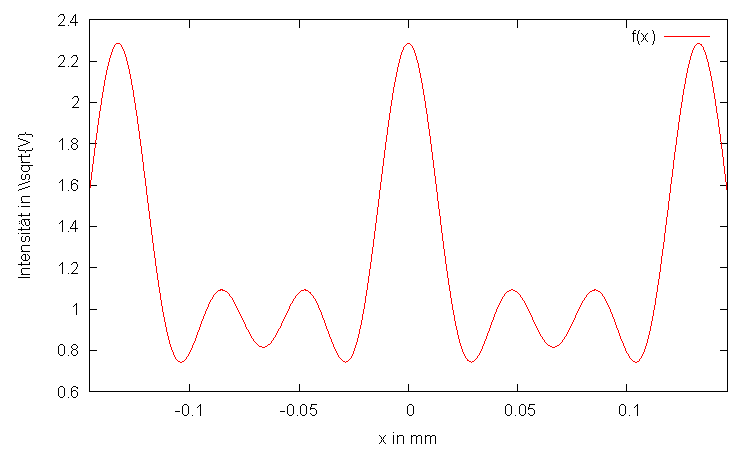
\includegraphics{Bilder/appertur.pdf}
\caption{Apperturfunktion mit $K = 130.96 \mu m $}
\end{figure}


\subsection{Bestimmung des Verh\"altnisses zwischen Spaltbreite und Spaltabstand}

Wir erhalten für das Verhältnis von Spaltbreite zu -höhe
$$ v = \frac{b}{K-b} = 0.26378 $$ %TODO Fehler? 

\subsection{Aufl\"osungsverm\"ogen der Gitter}

Für das Auflösungsvermögen der Gitter haben wir erhalten:

\begin{itemize}
\item Gitter 1: $ a = 67.765 \pm 11.302 $
\item Gitter 3: $ a = 56.437 \pm 9.407 $
\item Gitter 4: $ a = 28.294 \pm 4.715 $
\item PHYWE 08540: $ a = 28.566 \pm 4.764 $
\item PHYWE 08534: $ a = 45.816 \pm 7.636 $
\end{itemize}


\subsection{Raman-Nath-Theorie}

Wir konnten die Raman-Nath-Theorie für die 0. bis 2. Ordnung bestätigen, höhere Ordnungen konnten wir nicht (hinreichend häufig) auflösen.

\subsubsection{Ultraschallwellenlänge}

Für die Ermittlung der Schallwellenlänge haben wir die Messung bei $ U = 9.69 V$ und $f = 2109.195 kHz $ verwendet und  
$$\boxed{ \lambda^* = (575.329 \pm 2.6\e{-6}) \mu m}$$
erhalten. Unser Ergebnis weicht 9\% vom theoretischen Wert $ \lambda^*_{theo} = 526.741 \mu m$ ab.
